\begin{figure}[H]
	\centering
	\begin{minipage}{\linewidth}
		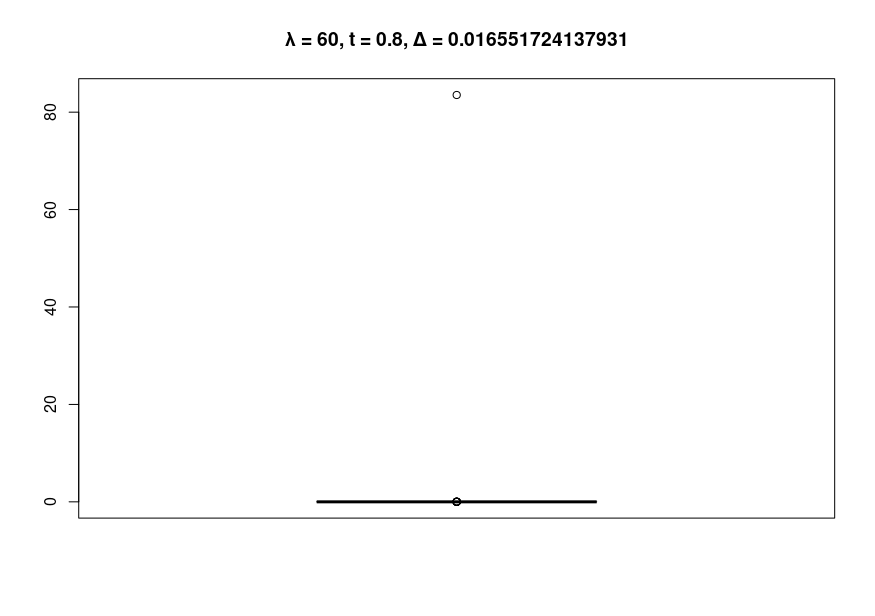
\includegraphics[width=0.47\textwidth]{Images/indiv_vs_glob/qq160.png}
		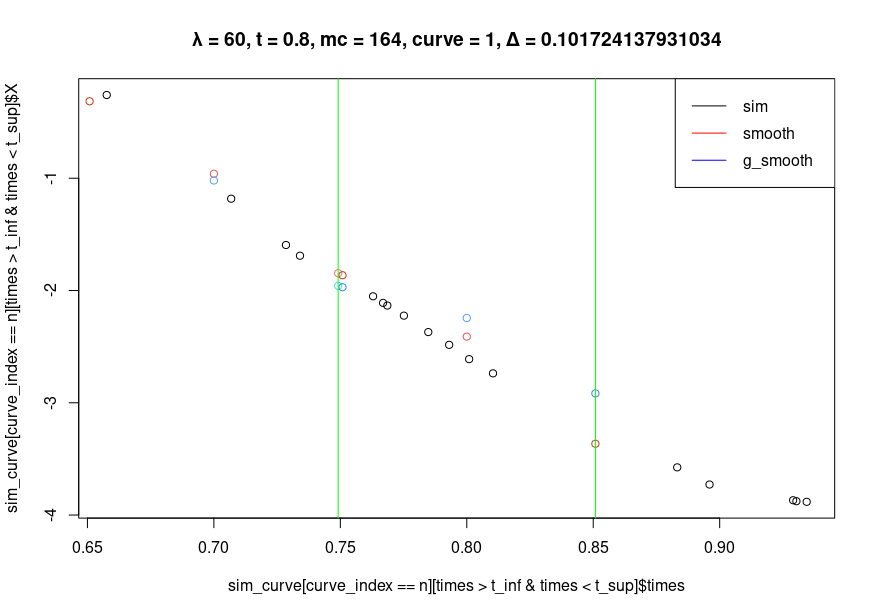
\includegraphics[width=0.47\textwidth]{Images/indiv_vs_glob/lbd60mc164c1.png}
	\end{minipage}

	\begin{minipage}{\linewidth}
		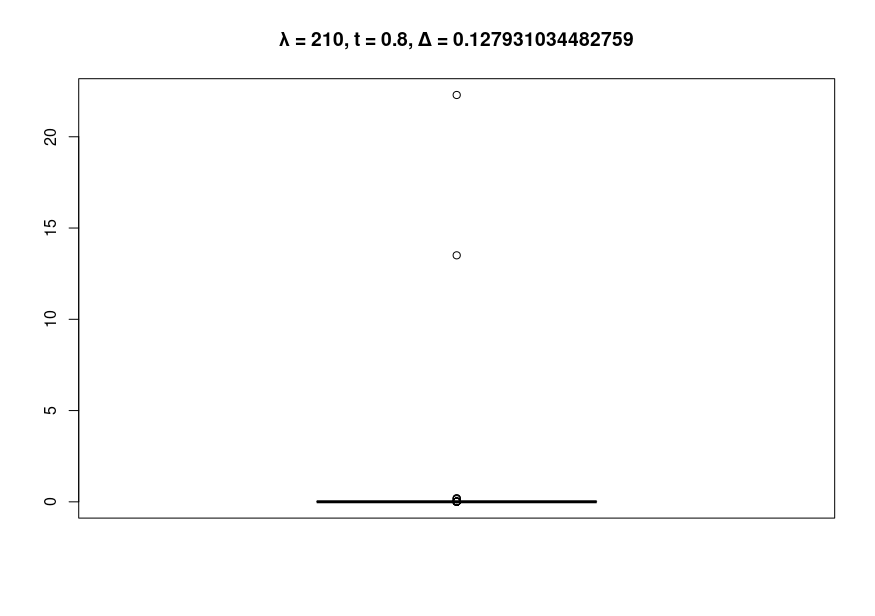
\includegraphics[width=0.47\textwidth]{Images/indiv_vs_glob/qq210.png}
		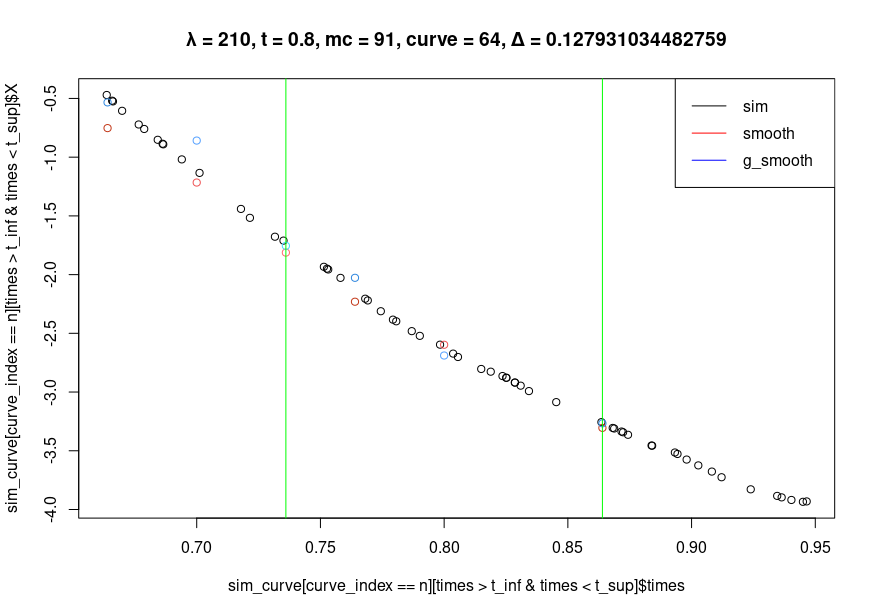
\includegraphics[width=0.47\textwidth]{Images/indiv_vs_glob/lbd210_mc91_c64.png}
	\end{minipage}
	\caption{Distribution des risques et aperçu d'une courbe pour un échantillon de monte carlo extrême sur le risque euclidien.}
	\label{fig:dist_R_eucl_curves}
\end{figure}

\begin{figure}[H]
	\centering
	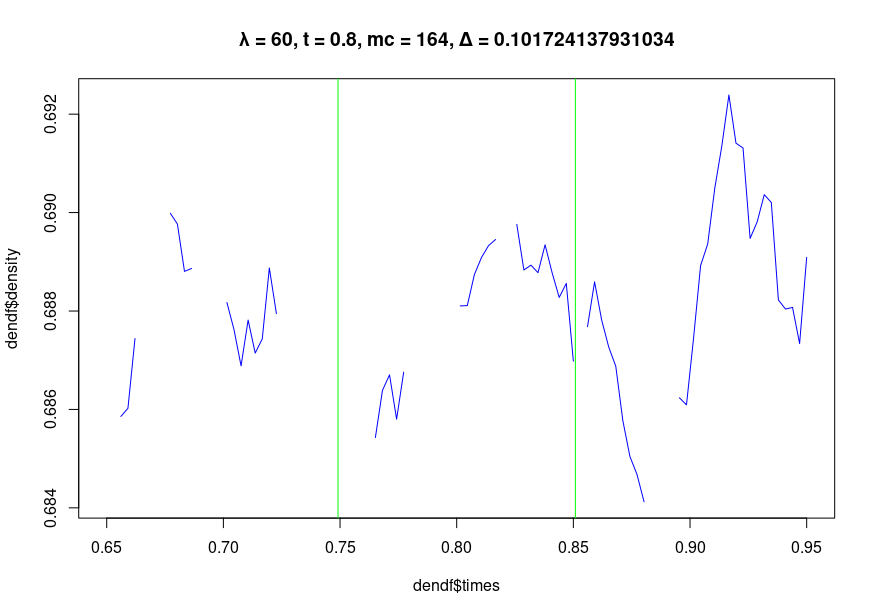
\includegraphics[width=0.7\textwidth]{Images/indiv_vs_glob/Tdensity_lbd60_mc164.png}
	\caption{Densité de points observés sur $[0.65, 0.95]$ pour $\lambda = 60$ sur un échantillon de monte carlo extrême, en un $\Delta$ problématique.}
	\label{fig:den_ex}
\end{figure}


\begin{figure}[H]
	\centering
	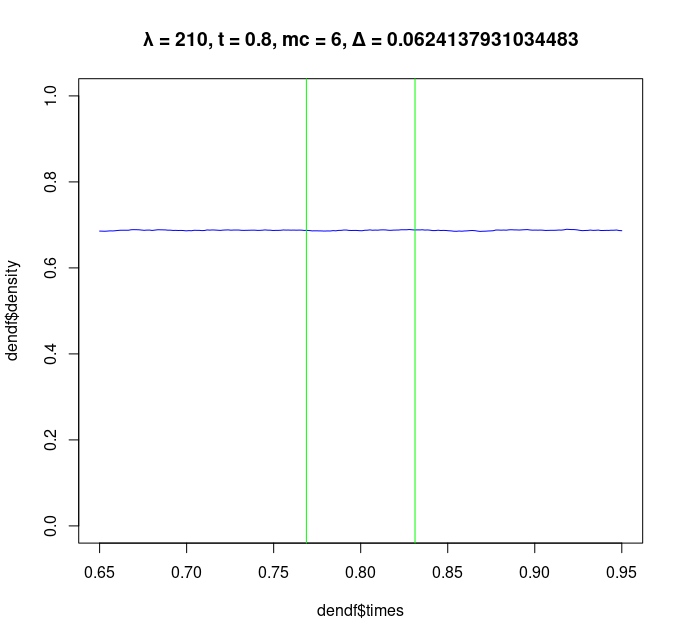
\includegraphics[width=0.7\textwidth]{Images/indiv_vs_glob/worst_210_67_mc6.png}
	\caption{Densité des points observés correspondant à la courbe présentée sur la figure \ref{fig:dist_R_eucl_curves}.}
	\label{fig:den_counterex}
\end{figure}



% N = 200	|
% λ = 90	|



% N = 200	|	
% λ = 210	|	


\begin{figure}[H]
	\centering

	\textbf{avec extrêmes : global}

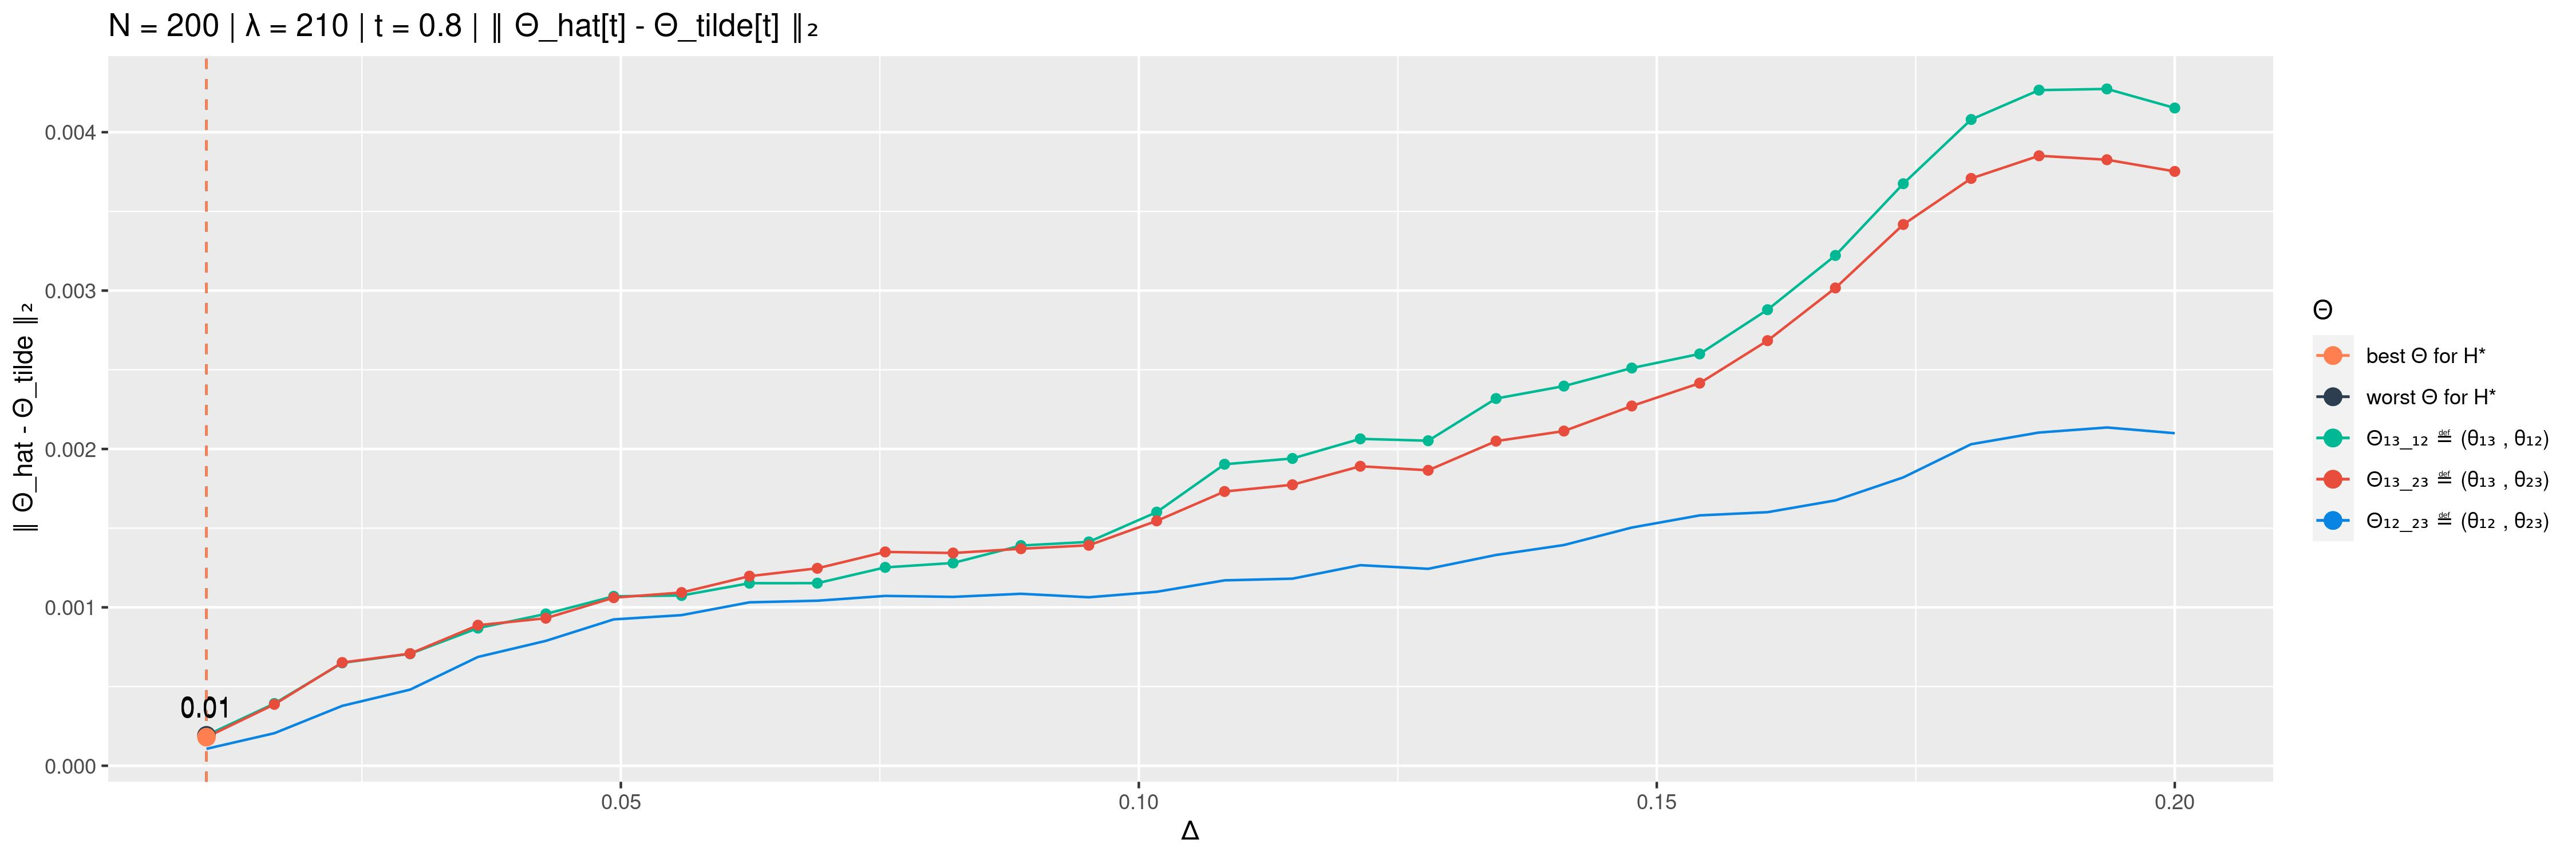
\includegraphics[width=0.9\textwidth]{Images/indiv_glob_img/compare/210_regular/all_glob.jpg}

	\textbf{avec extrêmes : individuel}

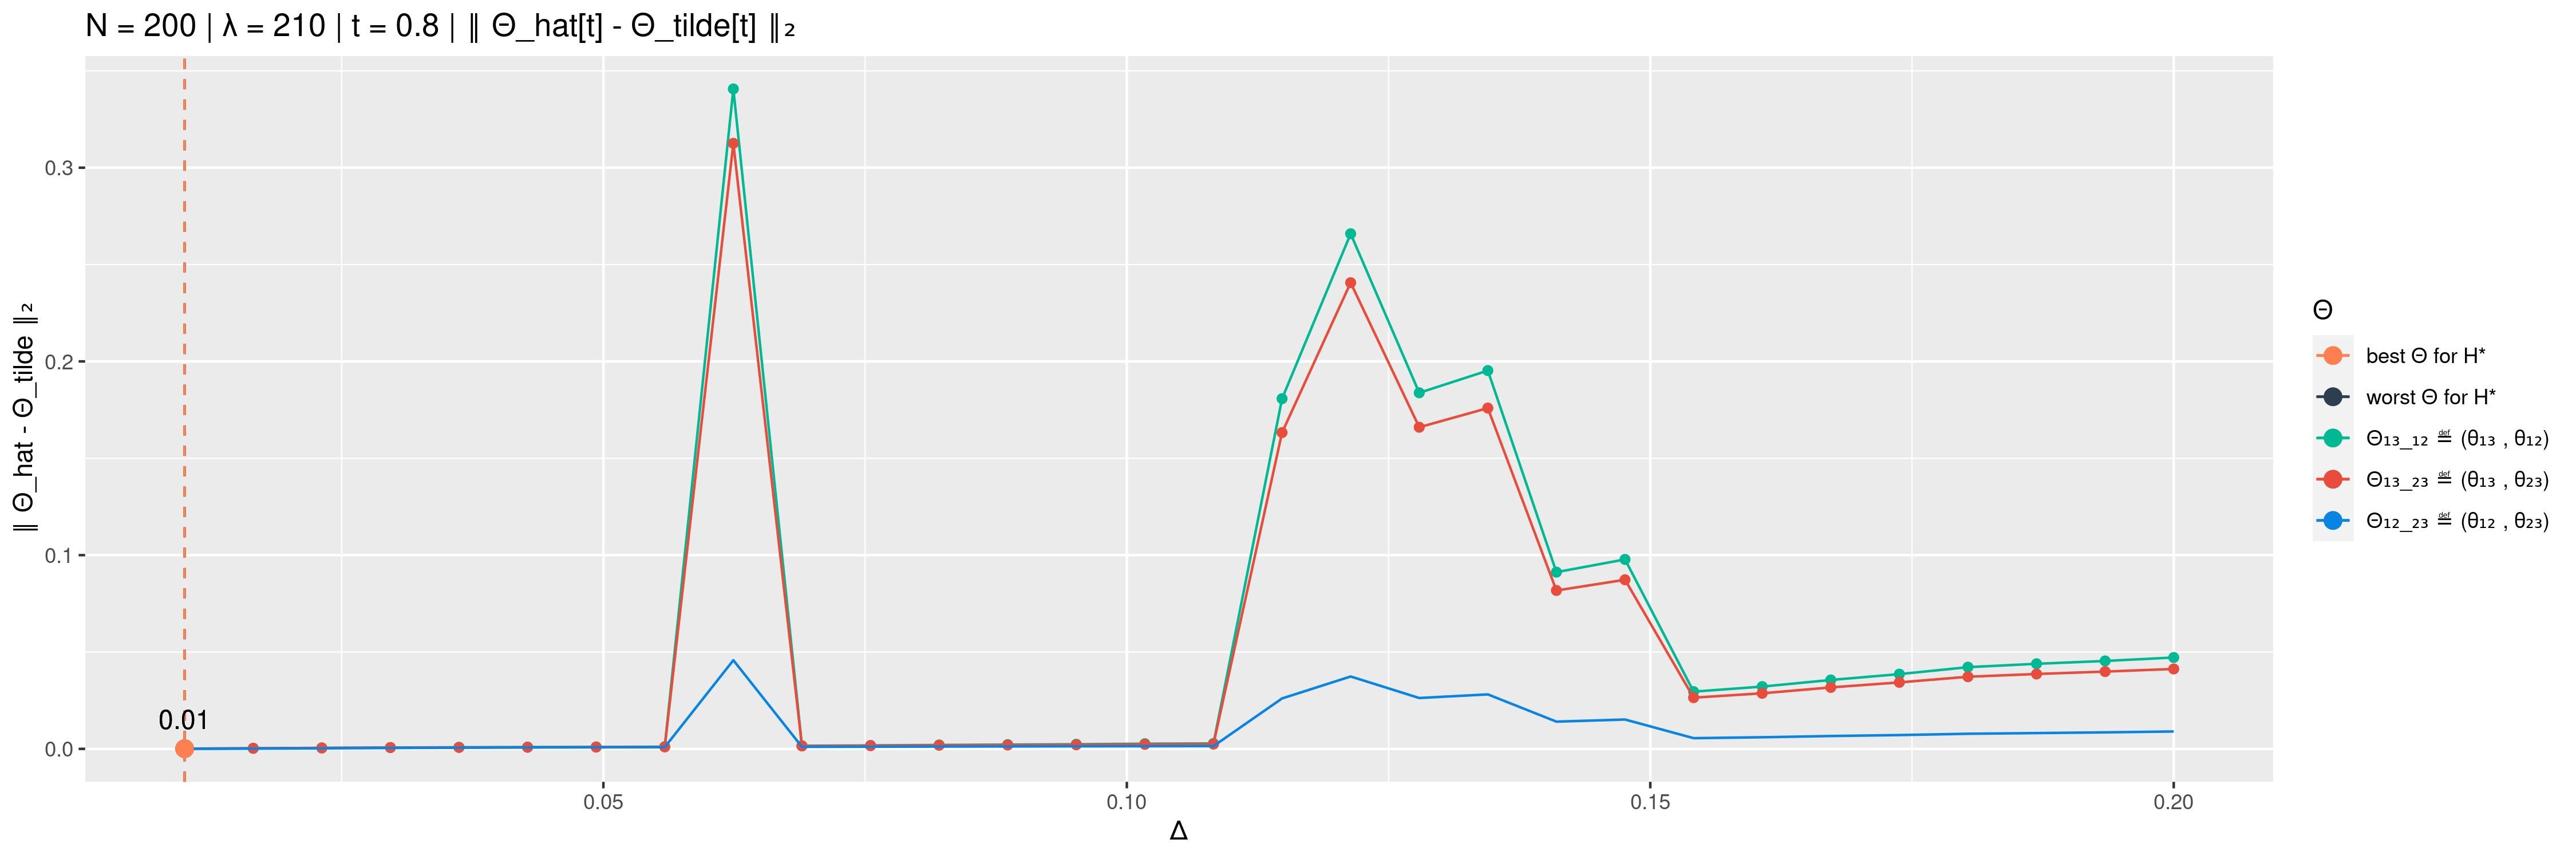
\includegraphics[width=0.9\textwidth]{Images/indiv_glob_img/compare/210_regular/all.jpg}

	\textbf{sans extrêmes : individuel} (- top 2\%)

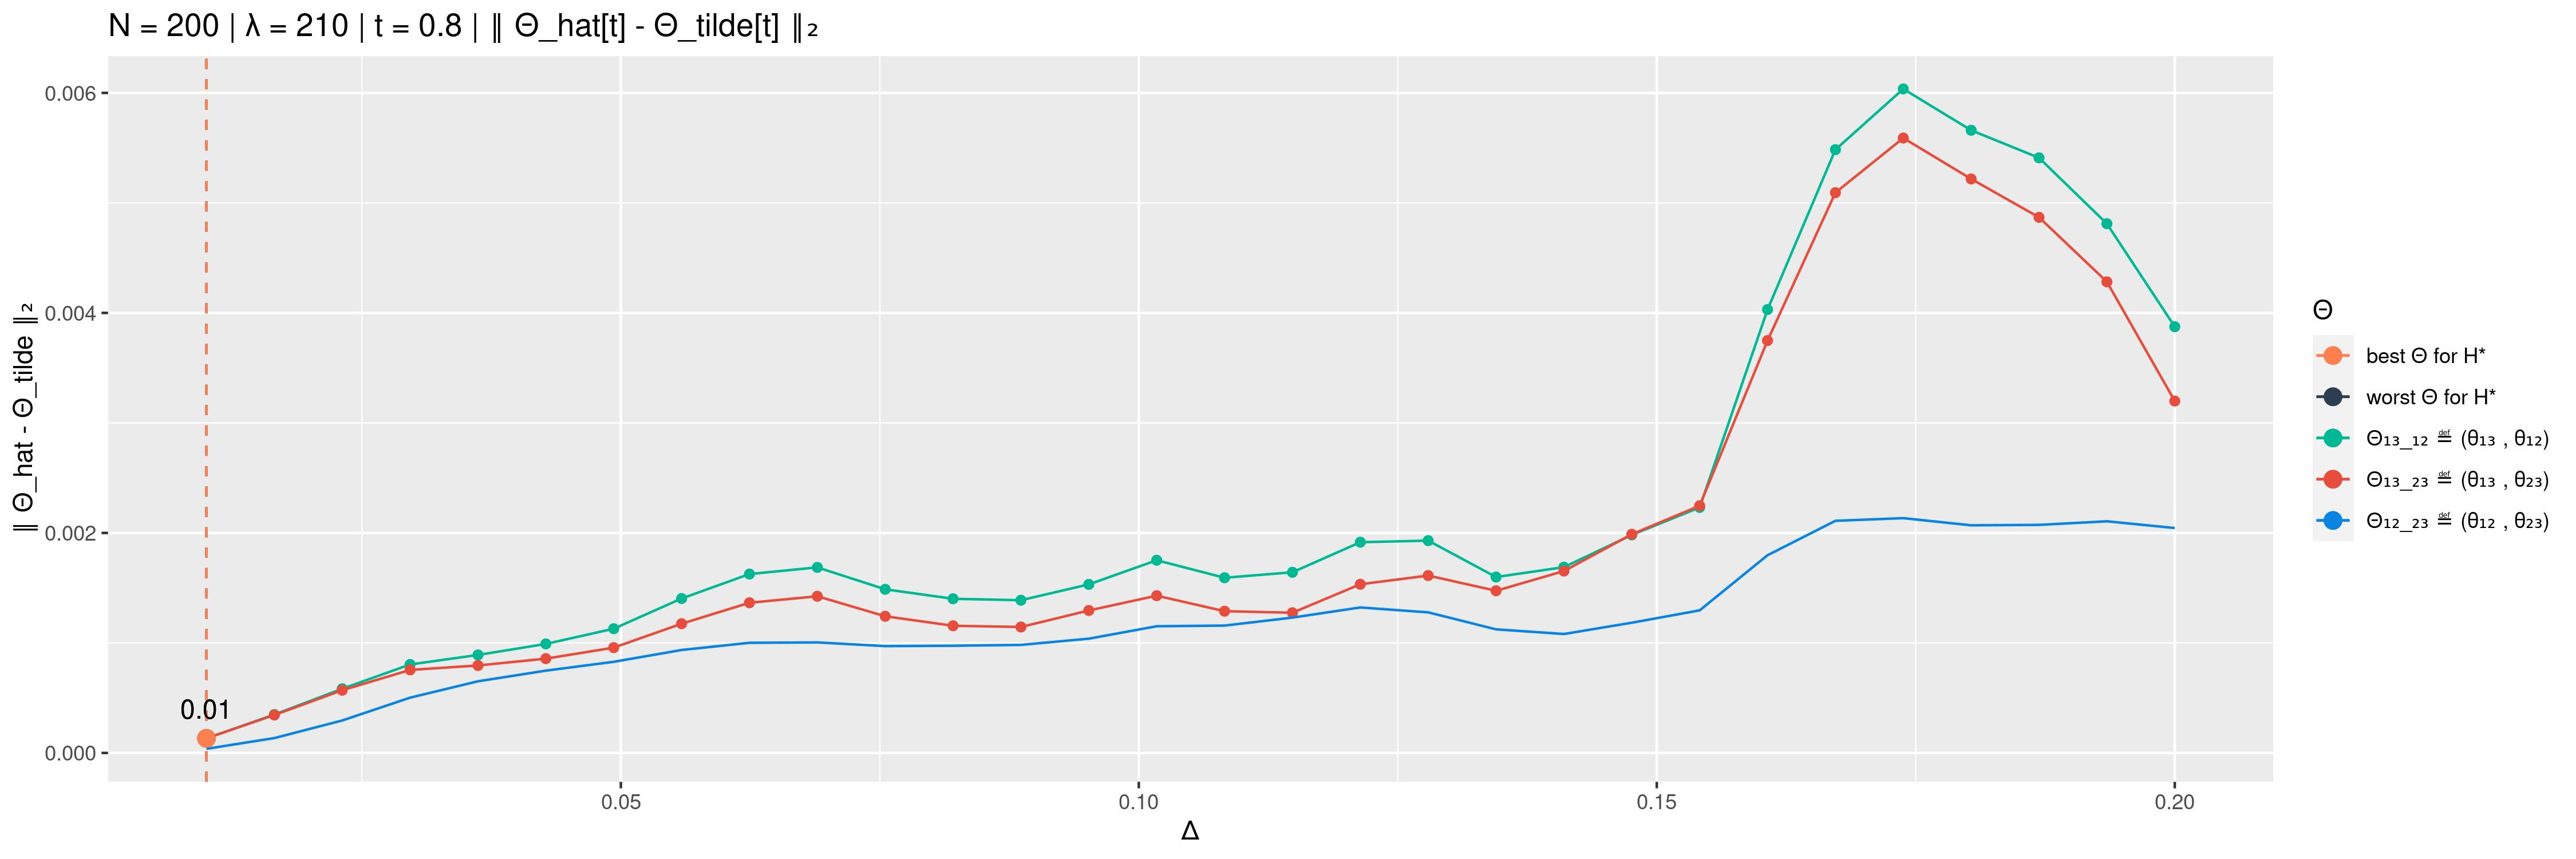
\includegraphics[width=0.9\textwidth]{Images/indiv_glob_img/compare/210_regular/no_xtrm.jpg}

	\textbf{sans extrêmes : global} (- top 2\%)

	% TODO : changer d image : mauvais N, prendre N=200
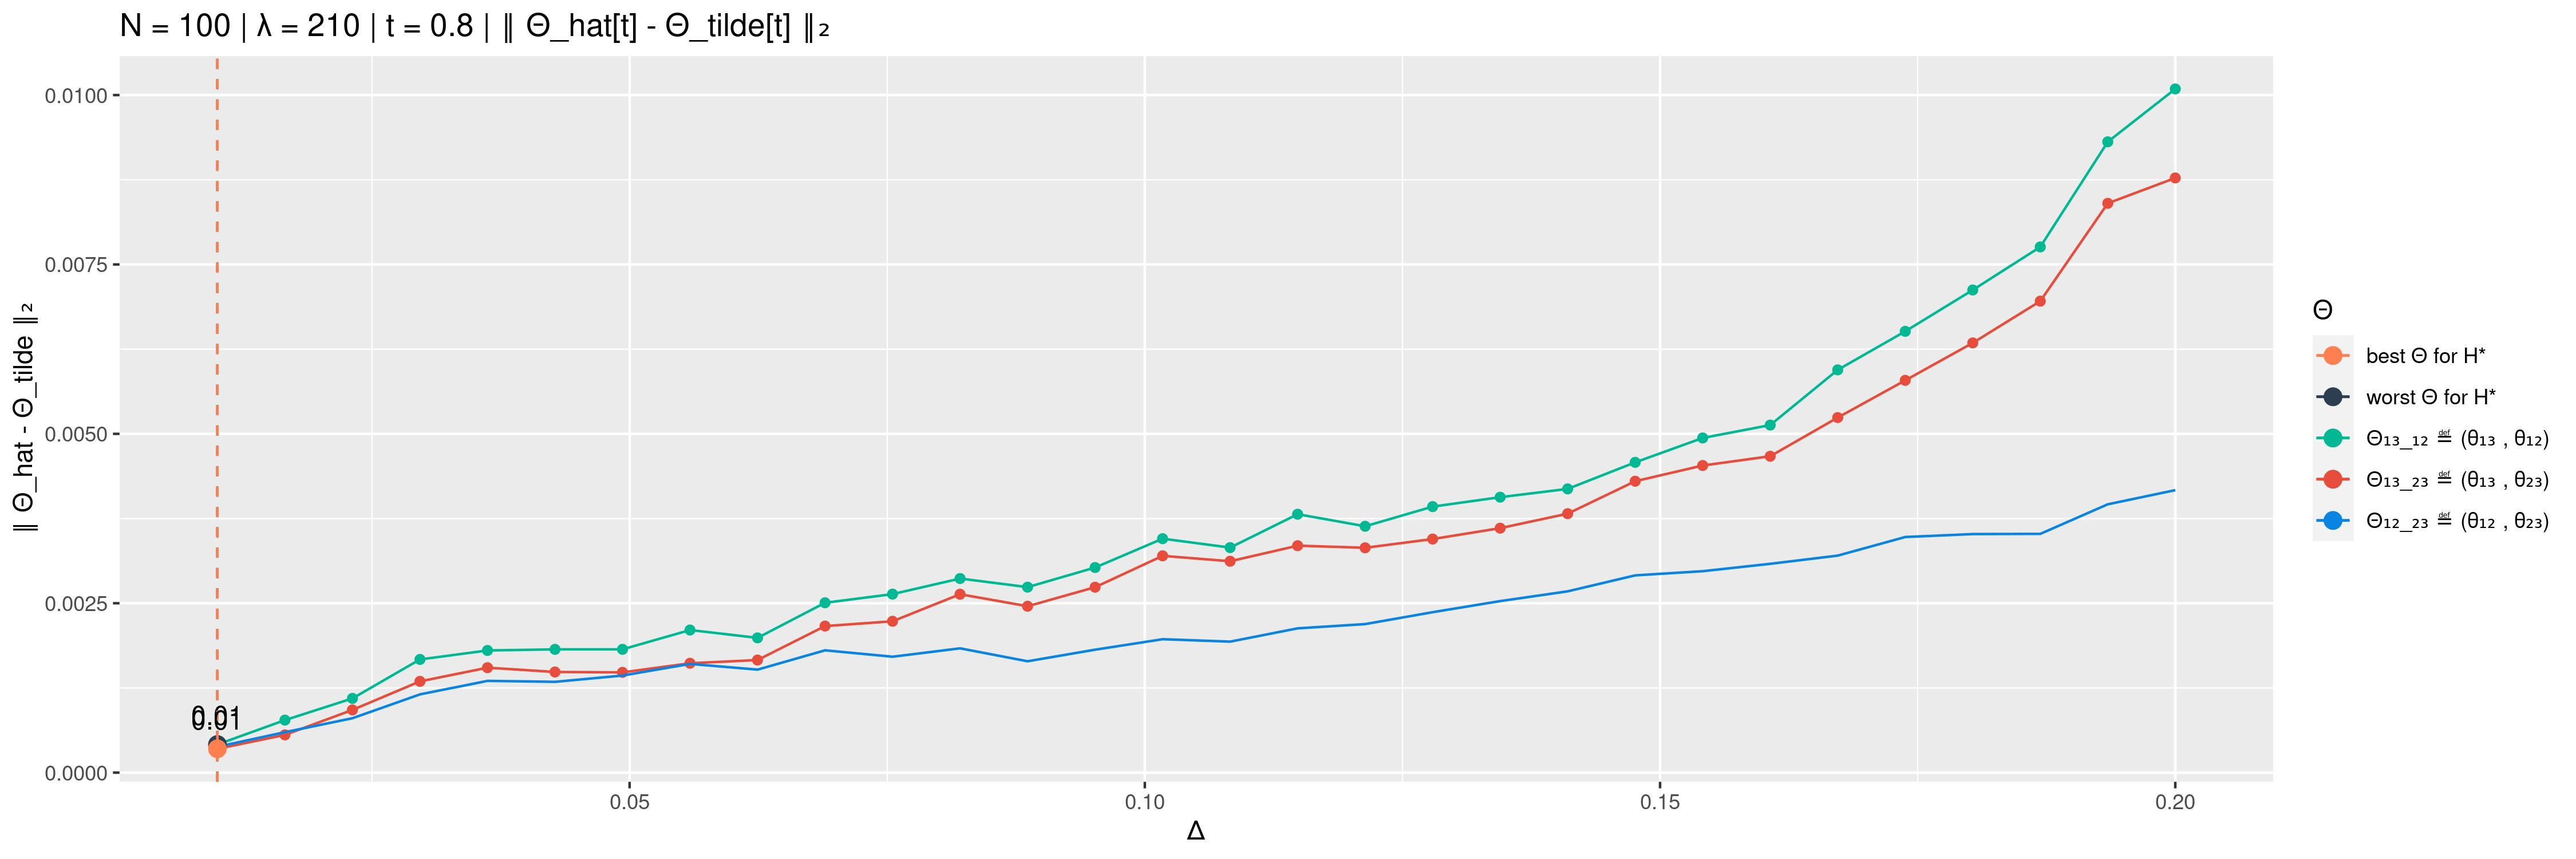
\includegraphics[width=0.9\textwidth]{Images/indiv_glob_img/compare/210_regular/no_xtrm_glob.jpg}
	\caption{Risque Euclidien pour $N=200$, $\lambda=210$ en un point régulier selon la méthode utilisée pour la fenêtre de lissage}
	\label{fig:compare_xtrm_2}
\end{figure}
